\documentclass[a4paper,12pt]{article}


%calling packages
\usepackage[english]{babel}
\usepackage[utf8]{inputenc}
\usepackage{amsmath}
\usepackage{graphicx}
\usepackage[left=1in,right=1in,top=1in,bottom=1in]{geometry}
\usepackage{setspace}
\usepackage[round]{natbib}
\usepackage{epstopdf}
\usepackage{soul}
\usepackage{lmodern}
\usepackage{caption}
\usepackage{hyperref}
\usepackage{subcaption}
\usepackage{lscape}
\usepackage{rotating}
\usepackage{etoc}


\usepackage{longtable}
\usepackage{amssymb}
\usepackage{fancyhdr}
\usepackage{array}
\usepackage{lscape} % for landscape formatting of pages
\newcolumntype{P}[1]{>{\centering\arraybackslash}p{#1}}
%fonts
\usepackage{times}
%\setcounter{secnumdepth}{0}
%chanfing font of table headers
\captionsetup[figure]{labelfont=bf}
\captionsetup[table]{labelfont=bf}

%path to where figures are located
\graphicspath{ {images/} }

%for notes in table captions 
\newcommand\fnote[1]{\captionsetup{font=small}\caption*{#1}}

%changing header
\pagestyle{fancy}
\fancyhf{}
\rhead{\thepage}
\renewcommand{\headrulewidth}{0pt}
\renewcommand{\footrulewidth}{0pt}
\renewcommand*\footnoterule{}
\let\svfootnoterule\footnoterule
\renewcommand\footnoterule{\vspace{0.2in}\svfootnoterule}
\renewcommand*{\thefootnote}{\fnsymbol{footnote}}
%set spacing

\renewcommand{\sfdefault}{phv}

\doublespacing
\usepackage{titlesec}

\titleformat*{\section}{\Large\sffamily}
\titleformat*{\subsection}{\large\sffamily}
\titlespacing*\section{0pt}{24pt plus 4pt minus 2pt}{4pt plus 2pt minus 2pt}
\titlespacing*\subsection{0pt}{20pt plus 4pt minus 2pt}{4pt plus 2pt minus 2pt}


%changing title settings
\makeatletter
\renewcommand{\maketitle}{
	\begin{flushleft}
		
		\onehalfspacing
		
		\@title
		
		\lineskip .5em
		\normalfont{\normalsize{\@author}}
\end{flushleft}}
\makeatother


\newcommand{\beginsupplement}{%
	\setcounter{table}{0}
	\renewcommand{\thetable}{S.\arabic{table}}%
	\setcounter{figure}{0}
	\renewcommand{\thefigure}{S.\arabic{figure}}%
}


%title
\title{\bigskip \bigskip \sffamily \LARGE{Can Citizens Set City Policy?} \\ \Large{ Evidence From A Decentralized Welfare State}}

%author
\author{\bigskip Benjamin Carl Egerod\footnote[2]{Graduate Student, Department of Political Science, University of Copenhagen, e-mail: \texttt{benjamin.carl.egerod@ifs.ku.dk}.} \qquad Martin Vinæs Larsen\footnote[3]{Assistant Professor, Department of Political Science, Aarhus University, e-mail: \texttt{mvl@ps.au.dk}.}} 

\usepackage{xr}
\externaldocument{"citypolicy"}


\begin{document}

	
	\begin{footnotesize} \noindent \today. \end{footnotesize} %date
	
\onehalfspacing


\renewcommand{\thesubsection}{\Alph{subsection}}
\renewcommand{\thetable}{\Alph{subsection}\arabic{table}}
\renewcommand{\thefigure}{\Alph{subsection}\arabic{figure}}

\section*{Appendix: For Online Publication}

\localtableofcontents

\clearpage


\subsection{Some More Context On Danish Municipalities} \label{context}
There have been two large reforms of local politics in the last 50 years. The first was conducted in 1970 as the Danish welfare state started to expand. Here the number of municipalities were reduced from more than 1000 to 275 \citep{ingvartsen1991kommunalreformen}. (Although it was 277 the first two years.)  The second reform was conducted in 2007 and further reduced the number of municipalities from 275 to 98. Once again, the increasing complexity of public service provision was a key argument for the reform \citep{christiansen2008utaenkelige}. Since both of these reforms were comprehensive in terms of amalgamations and changes to the relative power of national ctr. local government, we let them be the bookends of our analysis, examining the relationship between citizens policy views and the ideological flavor of municipal policy between the two reforms.\footnote{In this study, we exclude the municipality of Copenhagen and Frederiksberg, as these were governed in a different way.} Because of data availability we further limit our study period, so that it goes from 1978 and 2008.

In the period we study, Danish municipalities are governed by small city councils (between 9 and 29 members) which are elected at proportional elections and with a multi-party system which, to a large extent, mirrors the party system at the national level \citep{blom2013et}. Elections are fixed to take place every four years and do not usually coincide with elections at the national or EU level.\footnote{There was only three years between the elections of 1981 and 1978} Turnout is high with an average of around 70 percent since 1970.  

Following each municipal election, a majority in the city council elects a mayor, and the chairmen of the various committees \citep{serritzlew2008explaining}. Mayors are the only full time professional politicians in the city councils and have a number of formal obligations \citep{kjaer2015urban}. Mayors are also responsible for the day-to-day business of the administration and chairs the important economic committee which sets taxes and the budget. The work in the city council is structured by a a number of committees. The number and size of the committees is determined by the council. Committee membership is allocated proportionality between the political parties which means that there is broad political representation in all committees. The committees can decide on matters in their area and the administrative responsibility across areas is therefore essentially divided. 

\clearpage

\subsection{Overview of Policies Included in Our Measure} \label{policy}

%\begin{table}[h]
	\centering \footnotesize
	%\caption{Indicators of Fiscal Policy Conservatism}
	\label{tab:policies} 
	\begin{tabular}{p{5.5cm}P{3cm}P{4.5cm}} \hline
		\textbf{Policy}                          & \textbf{Availabiliy \newline (number of years)} & \textbf{Do Higher or Lower Values Imply Conservatism?} \\
		\hline
		&&\\ \textit{Tax policy} &&\\
		Income tax (pct.)                        & 29     &    Lower       \\
		Property tax (per mille)                      & 29    &    Lower        \\
		Commercial real estate tax (per mille) & 14    &    Lower               \\ \hline
	
		&&\\ \textit{Spending policy}  &&\\
		Spending pr. capita (DKK)                & 29    &    Lower        \\
		Spending pr. pupil in school (DKK)       & 7     &    Lower     \\ \hline
		
		&&\\\textit{Organization of public service delivery}  &&\\
 		Public Employees (pr. 1,000 citizens)	 & 9	  &	   Lower	     \\
 		Privately operated services  (pct.) &   14  &    Higher     \\
 		Purchases with a private supplier  (pct.)      & 14    &    Higher     \\ \hline
 	
 		&&\\ \textit{Co-payment for public services} &&\\   
		Average cost of day care (DKK)                  & 16    &    Higher     \\
		Price of relief stay (DKK)				 & 7	  &	   Higher	 \\
		Food delivery for the  elderly (DKK) & 7   &    Higher     \\
		Stay in nursing home (DKK)              & 7     &    Higher     \\ \hline
	
		&&\\ \textit{Extent of Public Services} &&\\ 
		Public housing (pct.)                    & 14     &    Lower               \\
		Class size in public schools	         & 14    &    Lower       \\
		\hline \hline
		\end{tabular}
\end{table} 

\clearpage

\subsection{Details about Estimation of Municipal Fiscal Policy} \label{estimation}

We parameterize fiscal conservatism using the following measurement model, which allows us to estimate it across time and space:

\begin{gather*}
F_{itk} \sim N(F^*_{itk}, \phi)\\
F^*_{itk} = \beta_k C_{it} - \alpha_{k}
\end{gather*}

Where $F$ is the level of the observed fiscal policy variable $k$ in municipality $i$ at time $t$. the distribution of each of these observed variables is drawn from a normally distributed latent variable $F^*$, which has variance $\phi$. $C$ is the quantity of most interest -- the latent fiscal conservatism in that municipality. $\beta$ is the discrimination parameter, which captures how strongly each observed policy variable loads onto the latent dimension. Finally, $\alpha$ represents each item's difficulty parameter, which measures how fiscally conservative a municipality is, if it were to score 0 on the policy variable $k$.

This parameterization is in many ways similar to frequentist factor analysis. However, a major advantage to using Bayesian techniques when making inferences about the latent trait is that the simulations will impute missing data during the estimation, which allows us to include items with different numbers of observations in the model -- the variables with missing observations will simply supply less information to the estimation. Additionally, the estimation is simulation based, which allows us to directly estimate uncertainty around all model parameters. 

We include the 14 policy variables listed in table  \ref{tab:policies} in the model. Before we do so, all variables are rescaled to have mean zero and variance one. Furthermore, all variables where higher values imply a more left-wing fiscal policy are reversed. This implies that when estimating policy conservatism, higher values on all variables indicate a more conservative policy. This is strictly speaking not necessary, but it makes interpretation of the model parameters simpler.

To identify the direction of the policy space, we constrain the $\beta$'s to be positive, so that municipalities scoring higher on our observed policy variables will be estimated to be more conservative. Location and scale is identified by placing standard normal priors on the distributions of all model parameters. All precision parameters are estimated using uninformative gamma priors.

Estimation is done by initiating a random walk over the parameter space defined by the model using the Gibbs sampler. We run 25,000 iterations of the model, where the first 2,500 are burn in. We run three parallel chains. To reduce autocorrelation within the chains of sampled values and improve convergence, we set a thinning interval of five, meaning that we only retain every fifth sampled value. Together, this specification ensured  convergence of the model and provided well-behaved, normal posterior distributions.

\clearpage

\subsection{Some Descriptive Features of Municipal Fiscal Policy} \label{descriptives}

Figure \ref{fig:descriptive} presents some descriptive features of the annual measure of fiscal policy conservatism. In particular, it looks at how the measure is distributed across time and space, revealing some interesting patterns in municipal fiscal policy.

Fiscal policy conservatism dropped slightly in the period. The drops are located in '78 to 81 and from 93 to 2000: periods where the Social Democratic Party was in power nationally. This makes sense as liberal national fiscal policies are likely to spill over into local politics through intergovernmental grants etc.

Aside from the national trends, however, the most notable feature of the time series seems to be the large variation we identify in fiscal policy. Some municipalities are, apparently, very fiscally conservative while others are very liberal. Although the within-differences are less dramatic, we also see some municipalities start out more conservative and then become more liberal and vice versa.

Further, the geographic spread of fiscal conservatism matches what most observers of Danish politics would expect. The most conservative municipalities are in Western Jutland and North of Copenhagen whereas the most Liberal (or Socialist) municipalities are west of Copenhagen and in an around the other large cities (Aaalborg, Aarhus, Odense). 
Figure \ref{mostleast} presents an overview of the most and the least conservative municipalities across the entire period.





\begin{sidewaysfigure}[htbp]
	\centering 
	\begin{subfigure}[h]{0.38\textwidth} 
		\includegraphics[width=1\textwidth]{newtimes_lines.eps}
		\caption{Average Municipal Fiscal Policy Conservatism (dark line) and Municipal Fiscal Policy Conservatism for Individual Municipalities (grey lines) from 1978 to 2006.}
		\label{fig:timeline}
	\end{subfigure} \hspace{1cm}
	\begin{subfigure}{0.38\textwidth} 
		\includegraphics[width=1\textwidth]{newJoyPlotFiscal.eps}
		\caption{Distribution of Municipal Fiscal Policy Conservatism from 1978 to 2006 (densities).}
		\label{fig:lines}
	\end{subfigure}
	\begin{subfigure}{0.9\textwidth} 
		\includegraphics[width=1\textwidth]{Map_of_FiscCon.eps}
		\caption{The Geographic Distribution of Municipal Fiscal Policy Conservatism at Three Points in Time.}
		\label{fig:map}
	\end{subfigure} 
	
	\caption{How has Municipal Fiscal Policy Conservatism Developed from 1978 to 2006?}
	\label{fig:descriptive}
	
\end{sidewaysfigure}

\begin{figure}
	\centering
	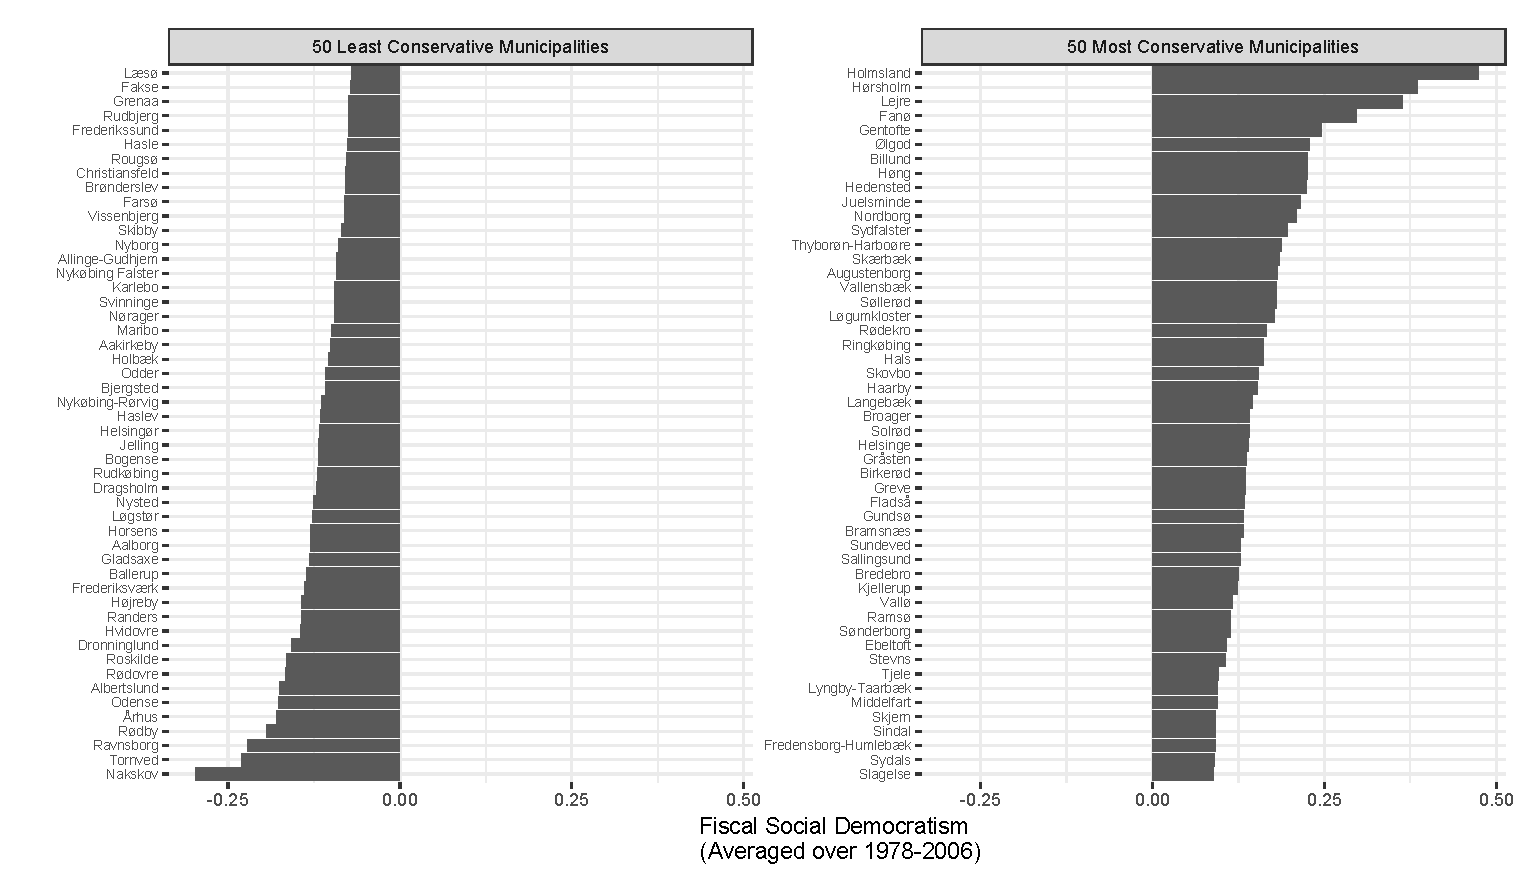
\includegraphics[width=1\textwidth]{socialdemocratism.eps}
	\caption{The Most and Least Conservative Municipalities} \label{mostleast}
\end{figure}

\clearpage


\subsection{Validating Our Measure Of Citizens' Policy Preferences} \label{validation}
In figure \ref{validation2}, we gauge the extent to which it matters that our measure relies on data from municipal rather than national elections. To do this, we correlate  municipal-level net support for conservative parties at the 2005 municipal election with municipal-level net support for the same conservative parties at a national election held six months earlier. This analysis reveals a strong, but in no way deterministic, correlation of 0.56. Accordingly, we might miss meaningful variation, if we used election returns from national, rather than local, elections to estimate local policy preferences.

\begin{figure}[htbp]
		\begin{subfigure}{0.45\textwidth}
		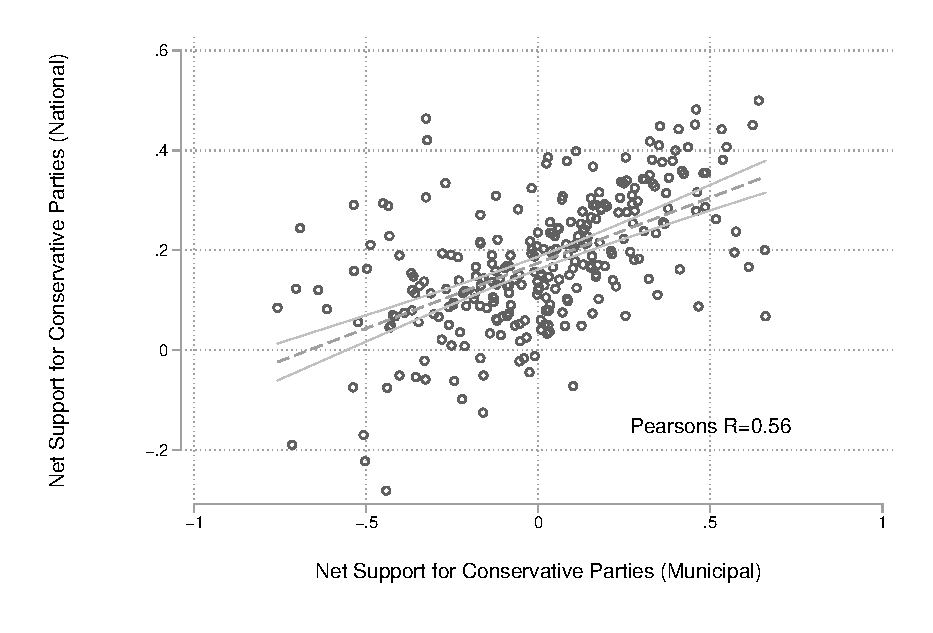
\includegraphics[width=1\textwidth]{validation2.eps}
		\caption{How strongly correlated are the electorate's preferences at municipal and national elections? Data from the 2005 municipal and national elections.} \label{validation2}
	\end{subfigure}
	\begin{subfigure}{0.45\textwidth}
		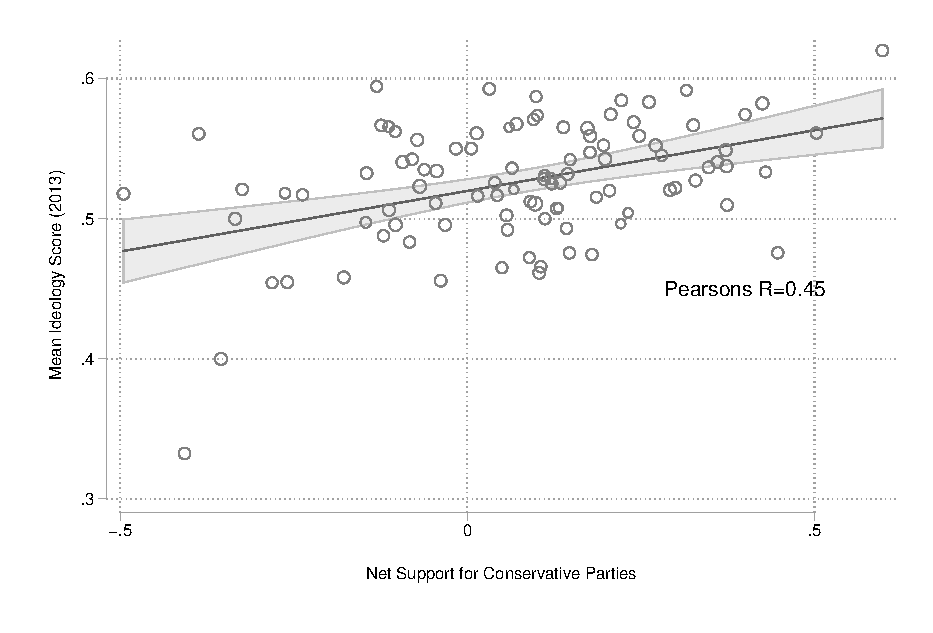
\includegraphics[width=1\textwidth]{validation.eps}
		\caption{Does the electorates preference over parties reflect preferences over policy? Data from the 2013 municipal election.} \label{validation1}
	\end{subfigure}  \hfill
	\caption{How does our measure of local policy preferences perform?}
\end{figure}

How well does this electoral measure capture voters underlying preferences? To get an indication of this, we look at the 2013 Danish Municipal Election Survey \cite{elklit2017kv13}. In this survey, more than 30 respondents (avg. 46) from each municipality were asked to place themselves on an eleven point ideology scale going from left to right. We calculate the municipality-specific mean of these responses and correlate these with the municipality-specific net support for conservative parties in the 2013 municipal election.  As can be seen from figure \ref{validation1}, the two are strongly correlated, which suggests that we are in fact tapping into relevant variation in policy views, when we measure citizens preferences over parties. Further, its important to note that the correlation is biased downwards, because we have random measurement error in our sample based measure of policy views.\footnote{The reader should also note that due to the municipal reform of 2006 (cf. the section on empirical context) we can only have 98 observations corresponding to the 98 (amalgamated) municipalities.}

\clearpage

\subsection{Regression Table for Main Results}

In Table \ref{main_res} we report a regression table summarizing  numerically the same information as the coefficient plot in the main text does graphically. Columns one through four use as the dependent variable the full measure of fiscal conservatism, while the remaining four columns use the reduced measure, which only include spending pr. capita, as well as taxes in income and property. All models include population size (logged) as a control. Column one shows the result from the pooled model, while column two includes twoway fixed effects. In the third column, we interact the time fixed effects with dummies for region and the log of population size. Finally, column four uses the first difference of all variables in the model instead of demeaning by municipality. Columns five through eight replicates these models with the reduced measure of fiscal policy conservatism. 

\begin{table}[!htbp] \centering 
	\caption{} 
	\footnotesize
	\label{main_res} 
	\begin{tabular}{@{\extracolsep{5pt}}lcccccccc} 
		\\[-1.8ex]\hline 
		\hline \\[-1.8ex] 
		& \multicolumn{8}{c}{\textit{Dependent variable:}} \\ 
		\cline{2-9} 
		\\[-1.8ex] & &\multicolumn{3}{c}{Full Measure$_{t+4}$} & &  \multicolumn{2}{c}{Spending Only$_{t+4}$} &  \\ 
		\\[-1.8ex] & (1) & (2) & (3) & (4) & (5) & (6) & (7) & (8)\\ 
		\hline \\[-1.8ex] 
		Right Vote & 0.416$^{***}$ & 0.129$^{***}$ & 0.145$^{***}$ &  & 1.110$^{***}$ & 0.317$^{***}$ & 0.335$^{***}$ &  \\ 
		& (0.059) & (0.037) & (0.048) &  & (0.122) & (0.081) & (0.099) &  \\ 
		& & & & & & & & \\ 
		FD Right Vote &  &  &  & 0.065$^{*}$ &  &  &  & 0.143$^{*}$ \\ 
		&  &  &  & (0.038) &  &  &  & (0.085) \\ 
		& & & & & & & & \\ 
		\hline \\[-1.8ex] 
		Municipality FE? & No & Yes & Yes & No & No & Yes & Yes & No \\ 
		Municipality FD? & No & No & No & Yes & No & No & No & Yes \\ 
		Time FE? & No & Yes & Yes & Yes & No & Yes & Yes & Yes \\ 
		Time X covariates? & No & No & Yes & No & No & No & Yes & No \\
		Observations & 1,908 & 1,908 & 1,908 & 1,363 & 1,908 & 1,908 & 1,908 & 1,363 \\ 
		R$^{2}$ & 0.057 & 0.874 & 0.924 & 0.672 & 0.071 & 0.843 & 0.914 & 0.869 \\ 
		Adjusted R$^{2}$ & 0.056 & 0.853 & 0.906 & 0.670 & 0.070 & 0.816 & 0.893 & 0.869 \\ 
		\hline 
		\hline \\[-1.8ex] 
		\multicolumn{9}{p{17 cm}}{\emph{Note: Robust standard errors with clustering at the municipality level are in parentheses. First-difference models uses Beck-Katz panel corrected standard errors. Population size (logged) included in all models.}} 
	\end{tabular} 
\end{table} 


\clearpage

\subsection{Does It Simply Reflect Fiscal Stress?}\label{balance}

In Table \ref{tab:balance}, we show how the electoral support for right-wing parties relates to changes in municipal socio-demographics. None of the correlations are strong. The largest coefficient is on percentage of college educated, where we estimate that an increase of one percentage point is related to a decrease in support for right-wing parties of approximately 1/20 of a standard deviation. Unsurprisingly, with these low correlations, we cannot reject the null that the coefficients individually nor collectively are zero. Besides this, it should be noted that the model's overall explanatory power is very low, as indicated by the negative adjusted $R^2$.

\begin{table}[!htbp] \centering 
	\caption{Support for Right-Wing Parties and Socio Demographics.} 
	\label{tab:balance} 
	\begin{tabular}{@{\extracolsep{5pt}}lc} 
		\\[-1.8ex]\hline 
		\hline \\[-1.8ex] 
		& \multicolumn{1}{c}{\textit{Dependent variable:}} \\ 
		\cline{2-2} 
		\\[-1.8ex] & Electoral Support for Right-Wing Parties \\ 
		\hline \\[-1.8ex] 
		Education & $-$0.007 \\ 
		& (0.005) \\ 
		& \\ 
		Immigrants & $-$0.0001 \\ 
		& (0.0001) \\ 
		& \\ 
		Unemployed & $-$0.003 \\ 
		& (0.002) \\ 
		& \\ 
		\hline \\[-1.8ex] 
		Wald Stat & 2.22 \\ 
		Municipality? & Yes \\ 
		Year FE? & Yes \\ 
		Observations & 818 \\ 
		Adjusted R$^{2}$ & $-$0.500 \\ 
		\hline 
		\hline \\[-1.8ex] 
		\multicolumn{2}{p{10 cm}}{\emph{Note: Robust standard errors clustered on municipality are in parentheses. P value for the wald statistic is 0.53.}}\\ 
	\end{tabular} 
\end{table} 
\clearpage

\subsection{Does Fiscal Policy Affect Voter Preferences?}\label{granger}

As an additional test for potential reverse causality, we use the lag of municipal policy as the explanatory variable in a series of fixed effects models predicting electoral support for right-wing parties. We use one through four year lags and report the result of each of these models in  \ref{fig:granger}. All coefficients are small, and we in none of the models can we reject the null that municipal policy does not predict voter behavior. This strengthens our claim that voter preferences explain policy and not the other way around.


\begin{figure}[!htb]
	\centering
	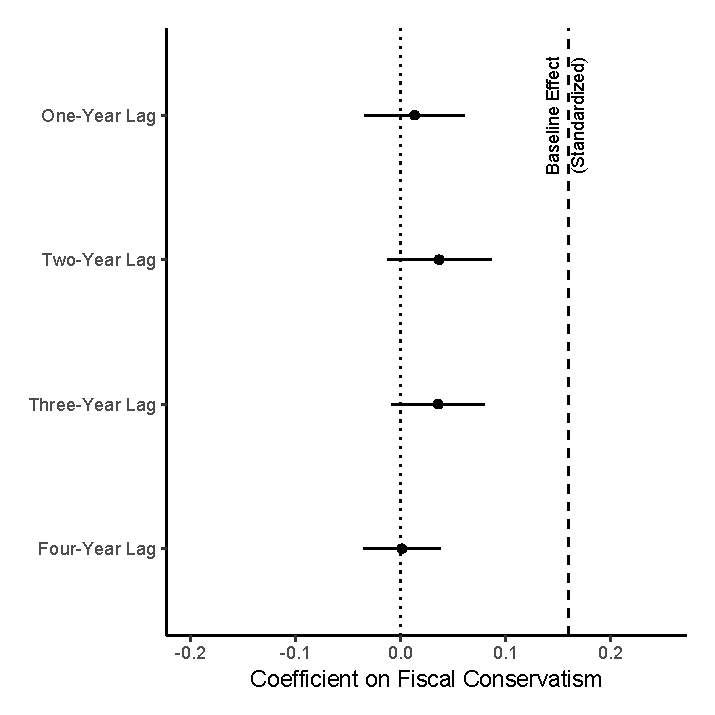
\includegraphics[scale = 1]{granger_18092018.eps}
	\caption{Reverse Causality? Fiscal Conservatism does not predict future support for Right-Wing parties. Confidence intervals are 95 percent, computed using robust standard errors clustered at the municipality level.} \label{fig:granger}
\end{figure}
\clearpage
\subsection{Is it Just The Mayoralty?}\label{mechanism}

There are two important reasons why we would expect municipal policy to be responsive to voter preferences. First, when the electorate chooses to elect more right-wing candidates, we would expect them to enact more fiscally conservative policies. Second, we might observe that parties are differentially responsive to voter preferences. We investigate these mechanisms in Figure \ref{fig:mech}.

In panel A, we include a categorical control for whether the mayoral party is the Liberal Party, the Social Democrats, or some third party.  In doing so, we condition the effect of electoral support for right-wing parties on, whether those parties control the most important municipal policy-making position. This gives us the effect of support for right-wing parties among the voters after taking into account, which politicians they elect. Identifying the direct effect of electoral support net of selection by including a post-treatment control in this way requires very strong assumptions that are unlikely to be met \textbf{REFERENCE}. Still, it is striking how little the coefficient on the policy preferences of the electorate changes, when controlling for the mayoral party. Additionally, it is interesting that policy does not seem to be different when the mayoralty changes from one party to another.

\begin{figure}[!htb]
	\begin{subfigure}{0.45\textwidth}
		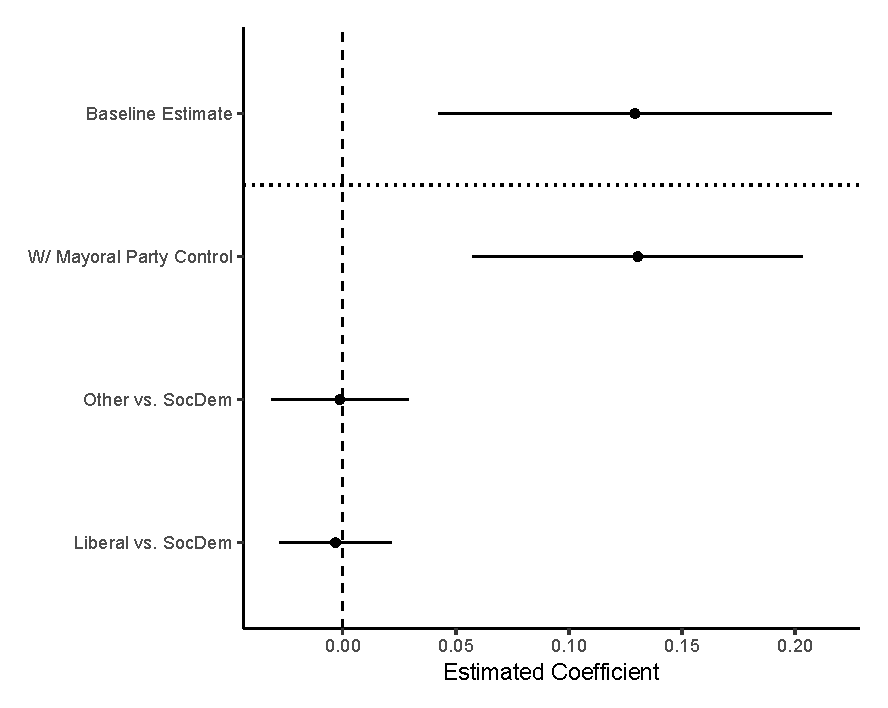
\includegraphics[width=1\textwidth]{PostTreatControl.eps}
		\caption{Are Results Driven by Selection? The figure shows results after including control for the mayoral party. Baseline estimates are included for comparison.} \label{mech}
	\end{subfigure}  \hfill
	\begin{subfigure}{0.45\textwidth}
		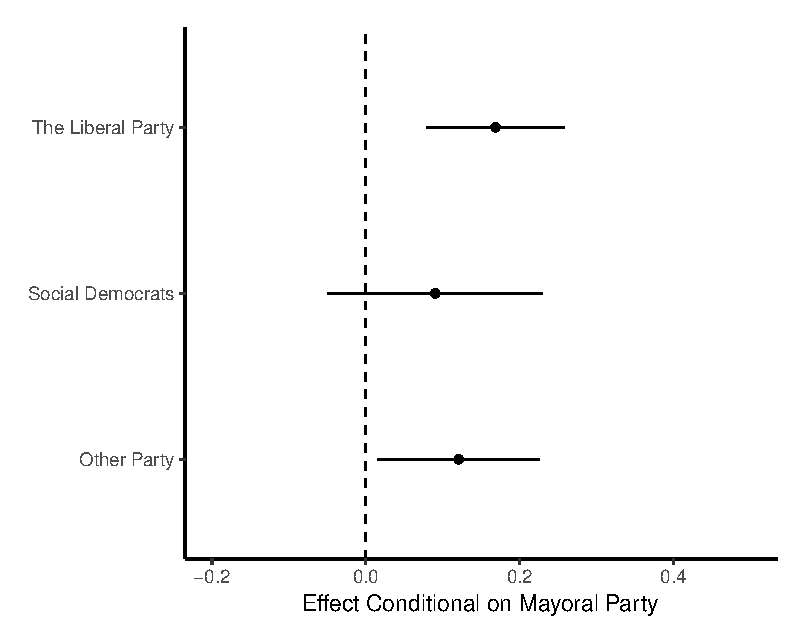
\includegraphics[width=1\textwidth]{MargFX_31082018.eps}
		\caption{Are All Parties Equally Responsive? The figure shows the marginal effects from a model including an interaction between mayoral party and electoral support for right-wing parties.} \label{inter}
	\end{subfigure}
	\caption{Responsiveness or Selection? Twoway fixed effects and population size (logged) included in both models. Confidence intervals are 95 pct., computed from robust standard errors with clustering at the municipal level.}
	\label{fig:mech}
\end{figure}

In panel B, we allow the effect to vary across our three different categories of mayoral party. The differences in the estimates are very small, and we cannot reject that policy under all three mayoralties respond equally to voter preferences.

\clearpage

\subsection{Effects on Individual Policy Indicators}


As our measure of municipal policy is made up of many different fiscal policies, it is interesting to investigate, which factor(s) drive the effect. The results of this exercise is reported in Figure \ref{fig:item} where we regress every single policy item in the measure individually on the electoral support of right-wing parties. While some of the variables are uncorrelated with voter preferences, the results also clearly show that a majority are strongly correlated with them, but many of them in a noisy manner. This suggests that combining the items has added value over only using one of them -- in this way, we can capture different aspects of municipal policy and also reduce the noise in the estimation. 

\begin{figure}[!htb]
	\centering
	
\includegraphics[scale = 1]{ItemByItem_18092018.eps}
	\caption{Effect of Right-Wing Electoral Support Across Components of our Measure. Note that all measures of taxes and spending are reversed to capture more conservative fiscal policies. Confidence intervals are 95 percent, computed using robust standard errors clustered at the municipality level.} \label{fig:item}
\end{figure}
\clearpage

\bibliographystyle{apa}
\bibliography{bibtex/library}


\end{document}